%%%%%%%%%%%%%%%%%%%%%%%%%%%%%%%%%%%%%%%%%%%%%%%
%%% Template for lab reports
%%%%%%%%%%%%%%%%%%%%%%%%%%%%%%%%%%%%%%%%%%%%%%%

%%%%%%%%%%%%%%%%%%%%%%%%%%%%%% Sets the document class for the document
% Openany is added to remove the book style of starting every new chapter on an odd page (not needed for reports)
\documentclass[10pt,english, openany]{book}

%%%%%%%%%%%%%%%%%%%%%%%%%%%%%% Loading packages that alter the style
\usepackage[]{graphicx}
\usepackage[]{color}
\usepackage{alltt}
\usepackage[T1]{fontenc}
\usepackage[utf8]{inputenc}
\usepackage{amsmath}
\setcounter{secnumdepth}{3}
\setcounter{tocdepth}{3}
\setlength{\parskip}{\smallskipamount}
\setlength{\parindent}{0pt}

% Set page margins
\usepackage[top=100pt,bottom=100pt,left=68pt,right=66pt]{geometry}

% Package used for placeholder text
\usepackage{lipsum}

% Prevents LaTeX from filling out a page to the bottom
\raggedbottom

% Adding both languages
\usepackage[english, italian]{babel}

% All page numbers positioned at the bottom of the page
\usepackage{fancyhdr}
\fancyhf{} % clear all header and footers
\fancyfoot[C]{\thepage}
\renewcommand{\headrulewidth}{0pt} % remove the header rule
\pagestyle{fancy}

% Changes the style of chapter headings
\usepackage{titlesec}
\titleformat{\chapter}
   {\normalfont\LARGE\bfseries}{\thechapter.}{1em}{}
% Change distance between chapter header and text
\titlespacing{\chapter}{0pt}{50pt}{2\baselineskip}

% Adds table captions above the table per default
\usepackage{float}
\floatstyle{plaintop}
\restylefloat{table}

% Adds space between caption and table
\usepackage[tableposition=top]{caption}

% Adds hyperlinks to references and ToC
\usepackage{hyperref}
\hypersetup{hidelinks,linkcolor = black} % Changes the link color to black and hides the hideous red border that usually is created

% If multiple images are to be added, a folder (path) with all the images can be added here 
\graphicspath{ {Figures/} }

% Separates the first part of the report/thesis in Roman numerals
\frontmatter


%%%%%%%%%%%%%%%%%%%%%%%%%%%%%% Starts the document
\begin{document}

%%% Selects the language to be used for the first couple of pages
\selectlanguage{english}

%%%%% Adds the title page
\begin{titlepage}
	\clearpage\thispagestyle{empty}
	\centering
	\vspace{1cm}

	% Titles
	% Information about the University
	{\normalsize Internet of Things \\ 
		Computer Science and Engineering \\
		Politecnico di Milano \par}
		\vspace{3cm}
	{\Huge \textbf{Third Homework}} \\
	%\vspace{1cm}
	%{\large \textbf{xxxxx} \par}
	\vspace{4cm}
	{\normalsize Erfan Rahnemoon 10720184 - 943057 \par}
	\vspace{5cm}
    
    \centering 
\includegraphics[scale=0.4]{logo1.pdf}
    
    \vspace{0.5cm}
		
	% Set the date
	{\normalsize 22-03-2020 \par}
	

\end{titlepage}

%%%%%%%%%%%%%%%%%%%%%%%%%%%%%%%%%%%%%%%%%%%%%%%%%%%%%%%%%%%%%%%%%%%%%%%%%%%%%%%%%%%%%%%%%%%%
%%%%%%%%%%%%%%%%%%%%%%%%%%%%%%%%%%%%%%%%%%%%%%%%%%%%%%%%%%%%%%%%%%%%%%%%%%%%%%%%%%%%%%%%%%%%
%%%%% Text body starts here!
%\mainmatter

\chapter{Summary}\label{chapt:sum}
[\textit{Answering some questions related to an analysis of the sniffed packets by Wireshark.}]
\newpage
\chapter{Questions ans Answers}
\section{What’s the difference between the message with MID:
3978 and the one with MID: 22636?}
We filter both packets with filter, \begin{equation*} coap.mid == 3978 || coap.mid == 22636 \end{equation*} and then we could show that the main difference is that the packet with MID=3978 is a confirmable packet that will have acknowledgment, but the message with MID=22636 is non-confirmable, so there is no ACK for it. Also, the value of SZX is different in both packets, which will determine the size of the packet.

\section{Does the client receive the response of message No.6949?}
Yes, if we get to the message with NO.6949, then we could filter with the MID of this message. \begin{equation*} coap.mid ==28357 \end{equation*} So we find the ACK packet of this message in the NO.6953. 

\section{How many replies of type confirmable and result code “Content” are received by the server “localhost”?}
By applying the following filter, we could see the number of packets is eight packets. The coap.type is set to 2  to find replies to confirmable type, and coap.code is set to 69 to find responses with a type of "content".
\begin{equation*}(coap.type == 2)\&\&(coap.code==69)\&\&(ip.dst == 127.0.0.1)\end{equation*}

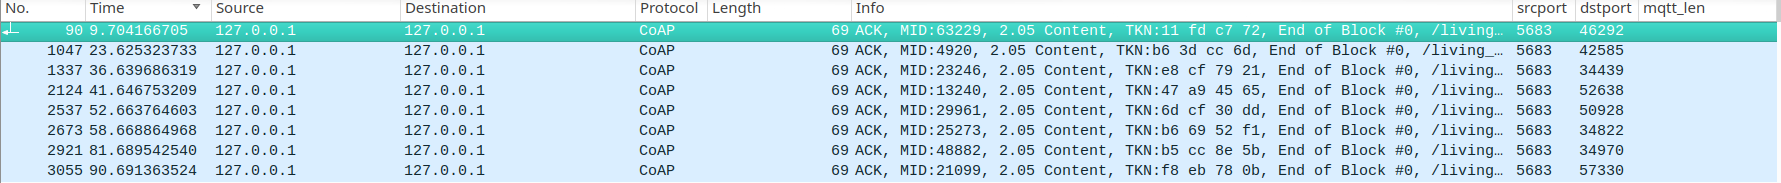
\includegraphics[scale=0.27]{3.png}

\section{How many messages containing the topic “factory/department*/+” are published by a client with user name: “jane”? Where * replaces the dep. number, e.g. factory/department1/+, factory/department2/+ and so on. (btw, * is NOT an MQTT wildcard)}
First, we find the packets that contain the username of "jane" to find the IP and port of the client used by "jane".
\begin{equation*}mqtt.username == "jane"\end{equation*}
Then we use the ports that we found from the previous filter to find all the packets sent by "jane".
\begin{equation*}tcp.srcport ==42821 || tcp.srcport==40989 || tcp.srcport==40005 || tcp.srcport==50985\end{equation*}
Finally, we update the previous filter to have the packets with the topic of "factory/department" and the type of published data that we should set mqtt.msgtype to three. Accordingly, the number of messages is six.
\begin{equation*}mqtt.msgtype==3 \&\& (tcp.srcport ==42821 || tcp.srcport==40989 || tcp.srcport==40005 || \end{equation*}
\begin{equation*}tcp.srcport==50985)\&\& mqtt.topic contains "factory/department"\end{equation*}
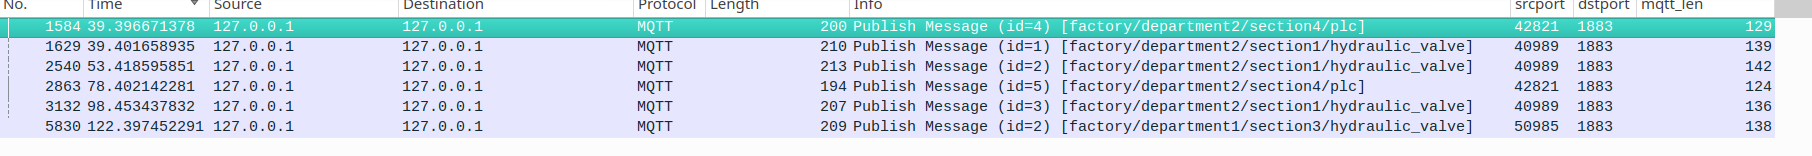
\includegraphics[scale=0.27]{4.png}


\section{How many clients connected to the broker “hivemq” have specified a will message?}
First, we filter packets with the following filter to find the DNS records related to “hivemq”.
\begin{equation*}frame\:contains\:hivemq\end{equation*}
Then, we use these IP addresses to find all the massages send for this broker. 
\begin{equation*}ip.dst==18.185.199.22 || ip.dst==3.120.68.56\end{equation*}
Next, we update the filter to find the messages with active Will flag; additionally, for being sure we have will\_mesaage in all of the messages, we could add mqtt.willmsg to the filter, but generally, the Will flag is enough.
\begin{equation*}(ip.dst==18.185.199.22 || ip.dst==3.120.68.56) \&\& mqtt.conflag.willflag == 1 \&\& mqtt.willmsg"\end{equation*}
Eventually, if we assume the client as one physical device with one IP address in the network, the number of connected clients is one. However, if we assume the client a program that is running on the physical machine, we will have 16 connected clients to the broker because we have 16 different source ports for the messages.

\section{How many publishes with QoS 1 don’t receive the ACK?}

To get the number of published messages with QoS set to one, we use the following filter that mqtt.msgtype is set to three, which means published packets. So the number of all published massages with QoS of one is 124.
\begin{equation*}(mqtt.msgtype == 3) \&\& (mqtt.qos == 1)\end{equation*}
Then we use the following filter to get the number of PUBACK (acknowledgment of publication packets) of publication with QoS of one, which is equal to 74 messages. The mqtt.msgtype is set to four because in MQTT specification for acknowledgment of Publication packets with QoS of one, the number 4 is used.
\begin{equation*}mqtt.msgtype == 4\end{equation*}
As we know, the QoS of one means at least once delivery so that some ACK may be duplicated, but by looking at port and ID of ACKs, we know that all of them are unique. Consequently, 124-74=50 publication packets are without ACK.

\section{How many last will messages with QoS set to 0 are actually delivered?}
In the beginning, we find messages with active Will flag and the Qos of zero by the following filter, which the number of them is equal to 19.
\begin{equation*}mqtt.conflag.willflag==1 \&\& mqtt.conflag.qos==0\end{equation*}
Now, by knowing the port and IP of the packets, we found in the first part, we filter ACK Connect messages by considering the QoS of zero means at most once delivery. 
We apply the next filter, and by the help of vertical line In the No. column, IPs, and ports, we find the ACK of each one and mark them. Also, the mqtt.msgtype equal to one means connect command and equal to two means the ACK of the command.
\begin{equation*}mqtt.msgtype==2 || mqtt.msgtype==1\end{equation*}

Finally, if we assume the three malformed ACK Connect packets are not acceptable, so we are sure 16 of these messages are delivered.

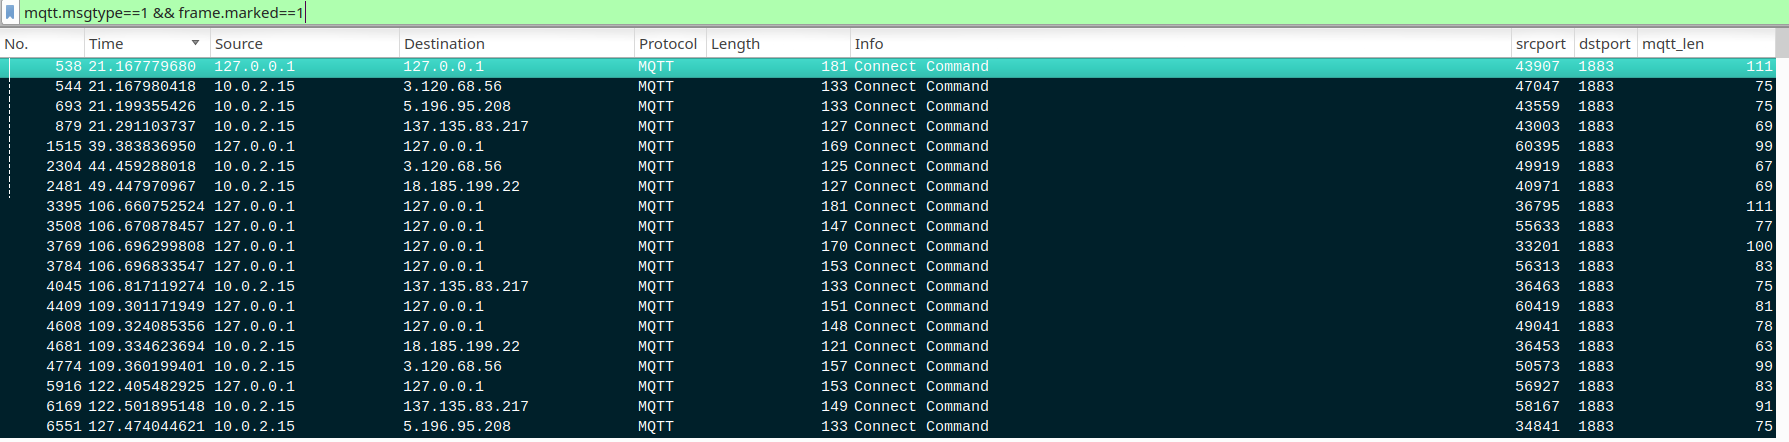
\includegraphics[scale=0.27]{7-1.png}

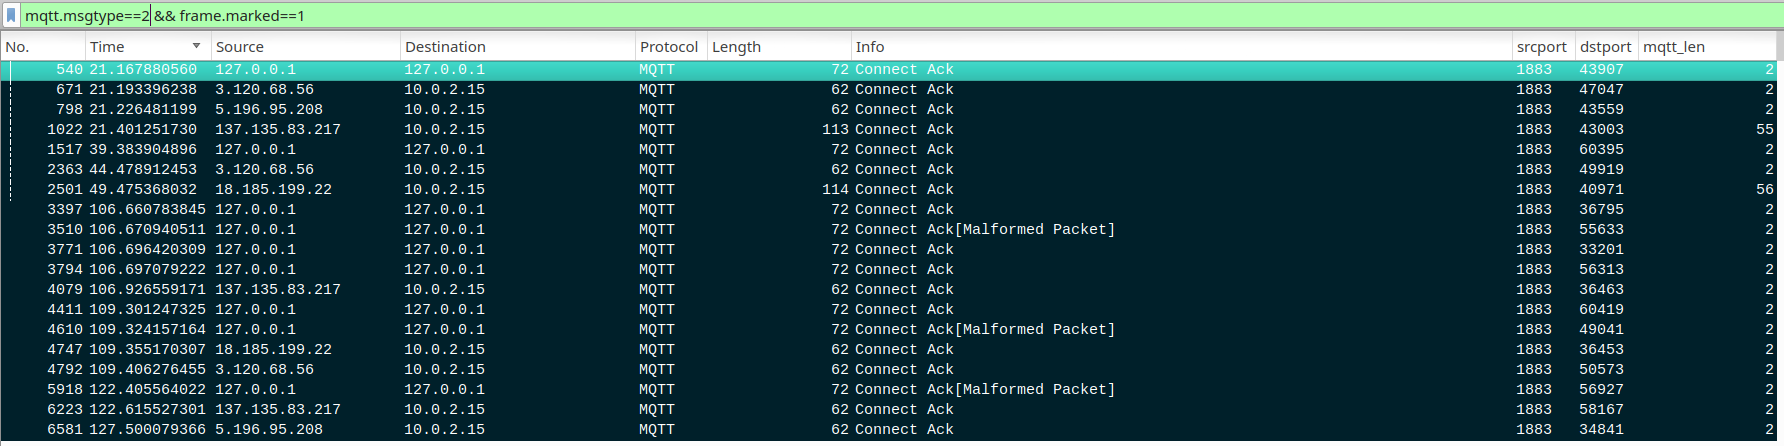
\includegraphics[scale=0.27]{7-2.png}


\section{Are all the messages with QoS > 0 published by the client\\ “4m3DWYzWr40pce6OaBQAfk” correctly delivered to the subscribers?}
First, we find the client's IP and ports by the next filter by using the client ID.
\begin{equation*}mqtt.clientid==4m3DWYzWr40pce6OaBQAfk\end{equation*}
Then we filter the messages send by the client which have the QoS of bigger than zero and the port and IP we found in the first part. 
\begin{equation*}ip.src==10.0.2.15 \&\& tcp.srcport==58313 \&\& mqtt.qos > 0\end{equation*}
After, we apply the following filter.(the mqtt.msgtype is set to five to find the Publish Received packets)
\begin{equation*}mqtt.msgtype == 5 \&\& tcp.dstport==58313\end{equation*}
We find only one Publish Received packet, so the subscriber receives the packet with No. 2423(Distinguishing packets by ID), but the receiver does not receive the packet with No. 968 correctly because there was no ACK for it even though the QoS is bigger than zero.

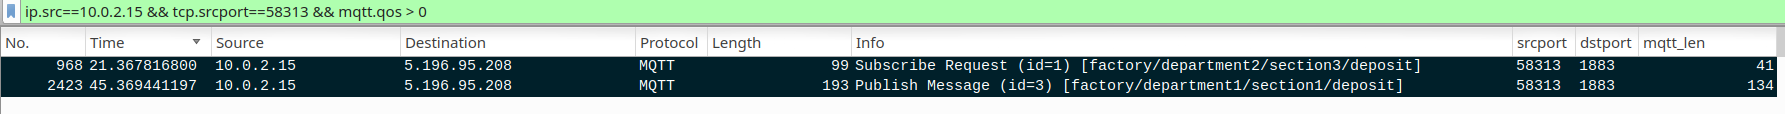
\includegraphics[scale=0.27]{8-1.png}

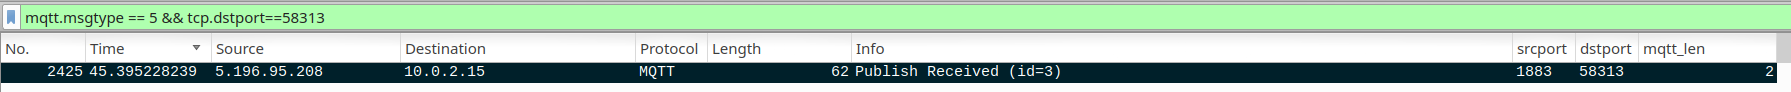
\includegraphics[scale=0.27]{8-2.png}

\section{What is the average message length of a connect msg using mqttv5 protocol? Why messages have different size?}
We use the following filter to find all the MQTT  Connect messages that the version is five.
\begin{equation*}(mqtt.ver==5) \&\& (mqtt.msgtype == 1)\end{equation*}
Then we use the mqtt.len as one column of Wireshark to find the massage length of each one and then calculate the average message length, which is 30.22. (In each multiplication, the first number is the number of the packet, and the second number is the length of the massage.)
\begin{equation*}((35 * 13) + (1 * 20) +(5 * 25) + (1 * 27) + (1 * 29) + (2 * 30) + \end{equation*}
\begin{equation*}(2 * 32) + (1 * 33) + (4 * 65) + (4 * 69) + (4 * 77) + (1 * 78) + \end{equation*}
\begin{equation*}(1 * 83) + (1 * 86))/63 = 30.222 \end{equation*}


The size of the message, depending on which flags are set, will vary a lot. For example, by setting the flag of Will the size of the packet could increase significantly by considering the size of the Will Topic and Will message. Also, the username and password flag could increase the size of the packet depending on the size of the username and password field, and client ID also increases the message length.

\section{Why there aren’t any REQ/RESP pings in the pcap?}
MQTT works on the TCP, and one of the TCP problems is the half-open connection to get around this problem. MQTT defines a field, which called keep-alive. Keep alive ensures that the connection between the broker and client is still open and that the broker and the client are aware of being connected.

The keep-alive is the duration in which the client and broker can send no message from the last transmitted message, and connection will be assumed open by both sides. In the absence of any message, the client and broker need control procedure to keep each other in check. This procedure is done by REQ/RESP pings.

For no REQ/RESP, there are two possibilities; first, the procedure is deactivated by setting the keep-alive to zero, which by checking the messages, we know that the keep-alive value is not zero. Second, As long as messages are exchanged frequently, and the keep-alive interval is not exceeded, there is no need to send an extra message to establish whether the connection is still open. The second possibility is the scenario that is happing in this sniffing, especially the duration of sniffing, is less than most of the keep-alive durations.
Also, of the frequent exchange of messages between broker and clients, we did not have the REQ/RESP.

\end{document}
